\clearpage
\section{Signal models and efficiencies\label{sec:signal}}

fill 

\subsection{Introduction}

As mentioned in section~\ref{theory}, SUSY is a theory of many particles
and parameters.  Simplifed models (SMS) have been derived~\cite{Alwall:2008ag,Alwall:2008va,sms}
which reduce both particles and parameters at the cost of losing 
generality of the full SUSY model. Yet, SMS models are benificial experimentally,
as they provide clear signatures to search for.  Two SMS models have been studied
1. T2cc: pair produced stop sparticles each decaying into a charm quark and a neutralino.
2. T2tt: pair produced stop sparticles each decaying into a top quart and a neutralino.

Event samples for the simplified models are generated by the CMS SUSY MC group
[REF] at leading order with \MADGRAPH~\cite{madgraph}. I%nclusive, process-dependent,
%next-to-leading order calculations with next-to-leading logarithmic
%corrections~\cite{susy-nlo-nll} (NLO+NLL) of SUSY production cross
%sections are obtained with the program \PROSPINO~\cite{Beenakker1996ch} and
%\verb!CTEQ6L!~\cite{Pumplin:2002vw} parton distribution functions. 
%The \texttt{FastSim} framework is used, and the simulated signal events
%include multiple interactions per LHC bunch crossing (pileup) with the
%distribution of reconstructed vertices that match the one observed in
%data.
The MC samples are listed in Section~\ref{sec:samples}.

The SMS samples are produced in bins of stop mass (mStop) and neutralino
mass (mLSP). The analysis efficieny is studied in the usual \njet, \nb binning
but due to computational limitations not all categories are used to set 
a limit on a given model. The choice of categories for a model is made by
computing the expected upper limit on the signal cross-section for each
category seperatly using the much quicker asymptotic method [REF]. The categories
are ranked by their expected upper limit. Depending on the number of 
mass bins and number of events per bin, two or more categories with the 
higest rank are chosen.

The simplified models, along with the event categories considered for each,
is summarised in Table~\ref{tab:simplified-models}.


\begin{table}[h!]
  \caption{A summary of the simplified models considered for
    interpretation. The event categories considered for each model are
    listed.}  
  \label{tab:simplified-models}
  \setlength{\extrarowheight}{2.5pt}
  \centering
  \begin{tabular}{ llcc }
    \hline
    \hline
    Model             & Production/decay mode & (\njet,\nb) event categories considered        \\ 
    \hline
    \texttt{T2cc}     & \Ttwocc               & (2--3,0), ($\geq 4$,0), ($\geq 4$,1) \\ % (2--3,1), 
    \texttt{T2tt}     & \Ttwott               & ($\leq 3$,1), ($\leq 4$,2) \\
    \hline
    \hline
  \end{tabular}
\end{table}

\subsection{Efficiency times acceptance\label{sec:t2cc-eff}}

The signal efficiency times acceptance is measured in the same binning
as the analysis binning (\njet,\nb,\scalht). To reduce the number of
figures in this section to a manageable level, the total efficiency for
only the relevant event categories and inclusive selection on 
\scalht ($>200\gev$) is shown. 
  
Figure~\ref{fig:sms-eff-t2cc} (Appendix~\ref{app:t2cc}) shows the
expected signal efficiency times acceptance for the hadronic selection
\texttt{T2cc} in the four most sensitive (\njet,\nb) event categories:
(2--3,0), (2--3,1), ($\geq 4$,0), and ($\geq 4$,1). 

\begin{figure}[h!]
  \begin{center}
    \subfigure[Hadronic Selection Efficiency, (2--3,0)]{
      \includegraphics[width=0.4\textwidth,page=6]{figures/sms/t2cc/v1/T2cc_eff}
    } 
    \subfigure[Hadronic Selection Efficiency, (2--3,1)]{
      \includegraphics[width=0.4\textwidth,page=7]{figures/sms/t2cc/v1/T2cc_eff}
    } 
    \subfigure[Hadronic Selection Efficiency, ($\geq 4$,0)]{
      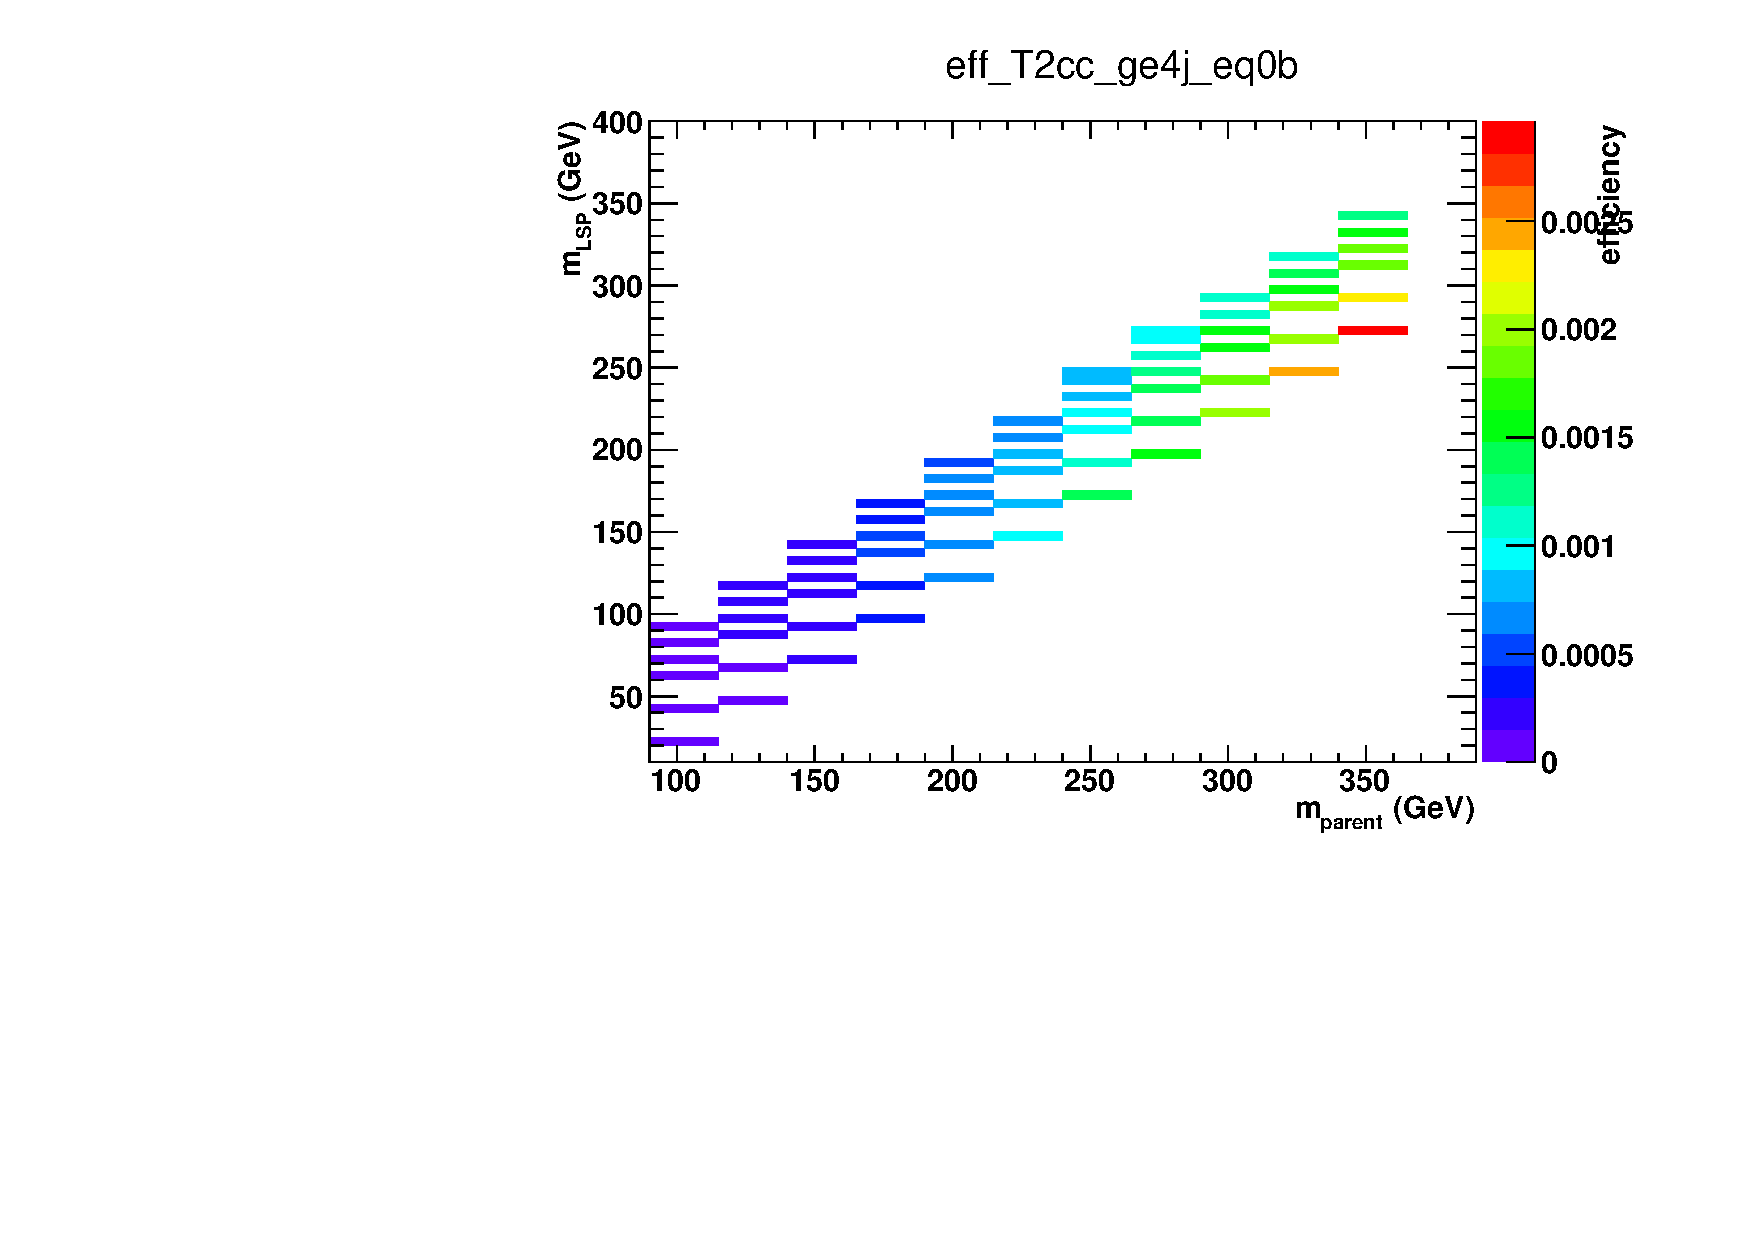
\includegraphics[width=0.4\textwidth,page=1]{figures/sms/t2cc/v1/T2cc_eff}
    } 
    \subfigure[Hadronic Selection Efficiency, ($\geq 4$,1)]{
      \includegraphics[width=0.4\textwidth,page=2]{figures/sms/t2cc/v1/T2cc_eff}
    } 
    \caption{Hadronic selection efficiency times acceptance for \texttt{T2cc}
      for the relevant event categories defined by \njet and \nb.
      Note the different z-axis scales.}
    \label{fig:sms-eff-t2cc}
  \end{center}
\end{figure}


%The choice of which categories to use is made by inspecting
%Figure~\ref{fig:sms-t2cc-sig} (Appendix~\ref{app:t2cc}), which shows
%the expected significance per signal region bin following the
%injection of signal at the theoretical QCD production cross section
%for the \verb!T2cc! model mass points $m_{\sTop} = 250\gev$ and
%$m_{\rm LSP} = 170\gev$ (Top) and $m_{\rm LSP} = 240\gev$ (Bottom).
%%$m_{\rm LSP} = 230\gev$ (Middle)

The efficiencies are typically at the percent level or less due to
reliance on hard-\Pt jets from initial state radiation for acceptance
in the presence of a compressed mass spectrum and soft decay
products. The largest efficiencies for the smallest mass splittings,
$\Delta M = \sim10\gev$, are obtained with the (2--3,0) category,
while for larger mass splittings the (2--3,1), ($\geq 4$,0), and
($\geq 4$,1) categories contribute due to the reduced backgrounds in
these categories. The signal efficiency in the \mj control sample is
negligible with respect to the signal region. By extension, the
relative contamination for the \mmj sample is also considered to be
negligible. Regardless, any potential contamination is accounted for
in the likelihood model.

%\subsection{Efficiency times acceptance for T2\_4body\label{sec:t2_4body-eff}}
%
%Figure~\ref{fig:sms-eff-t2_4body} (Appendix~\ref{app:t2_4body}) shows
%the expected signal efficiency times acceptance for the signal region
%and \mj control sample (\ie, signal contamination) for the model
%\verb!T2_4body! for the relevant event categories defined in terms of
%\njet and \nb. Several (\njet,\nb) categories are considered. As for
%\verb!T2cc!, the (2--3,0) category provides the largest efficiencies,
%typically at the percent level, for the smallest mass splittings. The
%(2--3,1), ($\geq 4$,0), and ($\geq 4$,1) categories contribute for
%larger mass splittings, but the efficencies are very low, typically at
%or below the per mille level, due to the presence of leptons in the
%final state. As a result, the signal contamination in the \mj and \mmj
%control samples, with respect to the signal region, can be
%non-negligible for models with larger mass splittings, but the S/B is
%still relatively small due to the increased background acceptance of
%the muon control samples (in the absence of an \alphat
%requirement). Further, any potential signal contamination is fully
%accounted for in the likelihood model.

\clearpage
\section{Systematic uncertainties on signal efficiency times 
  acceptance\label{sec:sms-syst}}

\subsection{Introduction} 

The systematic uncertainty in the signal acceptance times efficiency
is determined per mass point per event category (\njet,\nb), but inclusively
in \scalht to gain statistical power. This section details the methods 
used to determine the magnitude of the systematic uncertainties to be applied. 
Four sources of uncertainty are measured: the jet energy scale,
the parton distribution functions, initial state radiation and b-tag scale
factors. Two other uncertainties are quoted: the uncertainty in the luminosity
measurment and the ``dead ECAL'' filter used in the candidate signal
event selection. Each contribution is considered to be independent 
and all contributions are summed in quadrature to obtain a total 
systematic uncertainty per mass point per category.

The following sub-sections provide an overview of the various sources of
uncertainty, before details on specific models are provided. 
%
%\subsection{Shape systematics} 
%
%As stated above, the effect of various sources of uncertainty on the
%experimental acceptance times efficiency is determined per model per
%event category. However, some simplifications have been made in order
%to rationalise the process to determine the systematic uncertainties. 
%
%The systematic uncertainties presented below are determined per model
%per event category for an inclusive selection $\scalht >
%200\gev$. They reflect the effect on signal acceptance due to changes
%in the various sources of uncertainties. The resulting systematic is
%taken as a flat contribution across all \scalht bins for a given
%category. Clearly, this an overestimate for the higher \scalht bins,
%for which the probability to lose events (\ie fall below $\scalht >
%200\gev$) is significantly reduced. Further, events can migrate
%between (\njet,\nb) categories and not be lost, but again this
%approach does not account for category migration and overestimates the
%effect. Studies have been perform to check that the above approach is
%indeed appropriate, such as the effect of the dominant uncertainties
%(\eg JES, ISR, and PDF) on the \scalht shape for a model near to the
%expected limit contour. These studies are summarised below, which
%support the assumption that that systematic uncertainties in the
%signal acceptance times efficiency, if taken as a flat contribution
%across all \scalht bins, covers the uncertainty in the \scalht shape.
%
\subsection{PDF uncertainties\label{sec:pdf-sets}}

The simulated signal events were produced with the \verb!CTEQ6L1! PDF
set by default.  As recommended by PDF4LHC~\cite{pdf4lhc}, the uncertainty
in signal efficiency due to knowledge of the PDFs is obtained by comparing 
the signal efficiency with that obtained with three newer alternative PDF 
sets: \verb!CT10!, \verb!NNPDF2.1!, and \verb!MSTW2008!. Using the envelope
formula in the reference, a single value is calculated from the three alternate
PDF sets. Figures ~\ref{fig:sms-pdf-t2cc} and ~\ref{fig:sms-pdf-t2tt} in Appendix
 ~\ref{app:signal} summarize the uncertainty measured for T2cc and T2tt 
for the relevant categories. 

%\subsection{Jet energy scale\label{sec:sms-syst-jes}}
%
%The relative change in the signal efficiency times acceptance is
%determined when varying the energy of all jets in an event up or down
%according to a \pt- and $\eta$-dependent jet energy scale uncertainty
%(\ie vary the event scale up and down), as recommended by the JetMET
%POG. This procedure is followed per mass point per event category for
%an inclusive selection on \scalht ($> 200\gev$). 
%
%\subsection{Initial state radiation\label{sec:sms-syst-isr}}
%
%Signal samples are corrected to account for observed discrepencies
%with respect to data that are attributed to the mismodelling of
%initial state radiation in accordance with the procedure from the SUSY
%PAG~\cite{susy-isrrw}. In line with these corrections,
%sparticle-system \Pt dependent systematic variations are applied as
%shown in Table~\ref{tab:sms-syst-isr-factors}.  Events are reweighted
%according to the vectorial sum of the momenta of the pair-produced
%sparticles. In addition to the central weight, further variations
%about the central weight according to the uncertainty in the weight is
%applied in order to determine the systematic uncertainty associated
%with the correction. These systematic uncertainties are determined per
%mass point per event category for an inclusive selection on \scalht
%($> 200\gev$).
%The resulting systematic uncertainties are largest near the diagonal
%where selected events contain significant amounts of boost due to the
%presence of initial state radiation. 
%
%\begin{table}[!h]
%  \caption{Sparticle system \Pt dependent corrections and systematic
%    weight variations.} 
%  \label{tab:sms-syst-isr-factors}
%  \centering
%  \footnotesize
%  \begin{tabular}{ lcc }
%    \hline
%    Sparticle system \Pt (GeV) & Central Weight & Systematic Variation \\
%    \hline
%    $0 < \Pt < 120$            & 1.00           & $\pm$ 0.0            \\
%    $120 < \Pt < 150$          & 0.95           & $\pm$ 0.05           \\
%    $150 < \Pt < 250$          & 0.90           & $\pm$ 0.10           \\
%    $\Pt > 250$                & 0.80           & $\pm$ 0.20           \\
%    \hline
%    \hline
%  \end{tabular}
%\end{table}
%
%\subsection{b-tag scale factor corrections\label{sec:sms-syst-btag}}
%
%For the \verb!FastSim! signal simulation samples, the ``formula''
%method described in Section~\ref{sec:bjets} is not used and instead an
%event-by-event weight is applied directly to the simulated events
%following a prescription from the BTV POG. Furthermore, the use of the
%\verb!FastSim! framework in the reconstruction introduces an extra
%set of scale-factor corrections, to be applied simultaneously with
%those correcting the \verb!FullSim! simulation to the data.
%
%The magnitude of the corrections depends on the generator-level
%content, as well as the $b$-tagged status of the matched
%reconstruction-level jets. As an example, consider an event with 2
%generator $b$-jets matched to 2 reconstruction-level jets, of which
%only 1 fires the b-tagger, and 2 generator non-$b$-jets, also matched
%to 2 reconstruction-level jets, of which also only 1 fires the
%$b$-tagger. The probability for this to happen is given by:
%
%\begin{equation}
%  \begin{split}
%    P = \epsilon(p_{T}^{jet1}, \eta^{jet1}) \\ 
%    \times (1 - \epsilon(p_{T}^{jet2}, \eta^{jet2})) \\ 
%    \times m(p_{T}^{jet3}, \eta^{jet3}, ID^{jet3}) \\ 
%    \times (1-m(p_{T}^{jet4}, \eta^{jet4}, ID^{jet4}))
%  \end{split}
%\end{equation}
%
%where $\epsilon(p_{T}, \eta)$ and $m(p_{T}, \eta)$ are the $b$-tagging
%efficiency and mis-tagging rates respectively, as measured in the SM
%MC samples in a particular selection i.e. hadronic or muon, in a
%particular $H_{T}$ bin. The weight to correct this event is therefore
%given by:
%
%\begin{equation}
%  \label{equ:blah1}
%  w=\frac{SF_{b}\epsilon\times(1-SF_{b}\epsilon)\times SF_{c,light}m
%    \times (1-SF_{c,light}m)}{\epsilon\times(1-\epsilon)\times m \times
%    (1-m)} 
%\end{equation}
%
%where the relevant dependences are implied. Once all events have been
%reweighted this way, the yields in each $b$-tag bin represent the
%corrected MC yields. The scale factors in this case represent the
%scale factors from Ref.~\cite{btagpogtwiki} multiplied by the
%\verb!FastSim!-to-\verb!FullSim! correction factors. The
%\verb!FastSim!-to-\verb!FullSim! correction factors are summarised in
%\texttt{AN-2012-175}. The central value for these corrections is the
%same for all SMS samples, and is taken as the ratio between the
%effiency/mis-tagging rates of \ttbar samples produced with
%\verb!FullSim! and \verb!FastSim!. Similar to the differences between
%\verb!FullSim! and data, the b-tagging efficiency is higher in
%\verb!FastSim! than in \verb!FullSim! (thus needs a correction less
%than one), and the mistag rate is lower (thus needs a correction
%larger than one).
%%The 2011 recipe and values are unchanged in 2012.
%
%\subsection{\texorpdfstring{\mht/\met}{MHT/MET} cleaning cut\label{sec:sms-syst-mht-met}}
%
%%Figure~\ref{fig:mht-met-eff} compares the \mht/\met distributions
%%obtained from data and simulation in the \mj control sample with an
%%inclusive selection on \nb and $\scalht > 200\gev$, the requirement
%%$\alphat > 0.55$, and for the two jet multiplicity bins, \njetlow and
%%\njethigh. These samples largely comprises events from the W + jets
%%and \ttbar processes, which have significant, genuine \met. Hence, the
%%efficiency of the $\mht/\met < 1.25$ requirement is expected to be
%%high, and is indeed observed to be $>$95\%.
%
%The efficiencies observed in data and simulation for the requirement
%$\mht/\met < 1.25$ are summarised in Table~\ref{tab:mht-met} for the
%two jet multiplicity categories, \njetlow and \njethigh, and the
%analysis \scalht bins in the region $200 < \scalht < 375\gev$. These
%event samples comprise events from the W + jets and \ttbar processes,
%which have significant, genuine \met. Hence, the efficiency of the
%$\mht/\met < 1.25$ requirement is expected to be high, and is indeed
%observed to be $>$95\%. Also shown is the ratio of these two
%efficiencies, which should be unity. Any deviation from unity is taken
%to represent the uncertainties on the simulation modelling of this
%variable for processes with significant, genuine \met. The observed
%differences are at the percent level, demonstrating that the
%simulation models this variable to a level that is sufficient for this
%analysis.
%
%This approach covers the differences in the efficiencies determined
%from data and \verb!FullSim!. A further assumption is that the
%behaviour of the \mht/\met variable for simplified models produced
%with \verb!FastSim! is comparable to that for the dominant SM
%backgrounds, such as W + jets and \ttbar.
%
%\begin{table}[!h]
%  \caption{Efficiencies for the requirement $\mht/\met < 1.25$ obtained
%    from data ($\varepsilon_{\rm data}$) and simulation
%    ($\varepsilon_{\rm MC}$) in the \mj control sample with an
%    inclusive selection on \nb, the requirement $\alphat > 0.55$, for
%    the analysis bins at low \scalht, and for the two jet multiplicity
%    bins, \njetlow and \njethigh. Also quoted are the ratios of these
%    efficiencies ($\varepsilon_{\rm MC}/\varepsilon_{\rm data}$),
%    which is representative of the simulation performance with respect
%    to the \mht/\met variable.  
%  }
%  \label{tab:mht-met}
%  \centering
%  \footnotesize
%  \begin{tabular}{ ccccc }
%    \hline
%    \hline
%    \njet    & \scalht (GeV) & $\varepsilon_{\rm MC}$ & $\varepsilon_{\rm data}$ & $\varepsilon_{\rm MC}/\varepsilon_{\rm data}$ \\
%    \hline
%    2--3     & 200--275      & $0.95 \pm 0.00$        & $0.95 \pm 0.01$          & $1.00 \pm 0.01$                               \\
%    2--3     & 275--325      & $0.97 \pm 0.01$        & $0.97 \pm 0.02$          & $1.00 \pm 0.02$                               \\
%    2--3     & 325--375      & $0.97 \pm 0.01$        & $0.97 \pm 0.02$          & $1.00 \pm 0.02$                               \\
%    2--3     & 375--475      & $0.98 \pm 0.01$        & $0.98 \pm 0.03$          & $1.00 \pm 0.03$                               \\
%    $\geq 4$ & 200--275      & $0.90 \pm 0.02$        & $0.92 \pm 0.04$          & $0.98 \pm 0.04$                               \\
%    $\geq 4$ & 275--325      & $0.92 \pm 0.01$        & $0.93 \pm 0.02$          & $0.99 \pm 0.02$                               \\
%    $\geq 4$ & 325--375      & $0.92 \pm 0.01$        & $0.93 \pm 0.04$          & $0.99 \pm 0.04$                               \\
%    $\geq 4$ & 375--475      & $0.95 \pm 0.02$        & $0.95 \pm 0.04$          & $1.00 \pm 0.04$                               \\
%    \hline
%    \hline
%  \end{tabular}
%\end{table}
%
%\subsection{Dead ECAL filter\label{sec:sms-syst-dead-ecal}}
%
%The ratio of efficiencies observed in data and simulation for the dead
%ECAL filter are summarised in Table~\ref{tab:mht-met} for the two jet
%multiplicity categories, \njetlow and \njethigh, and an inclusive
%selection on \scalht ($>200\gev$). These event samples comprise events
%from the W + jets and \ttbar processes, which two dominant SM
%backgrounds for the signal region. Hence, the efficiencies of the dead
%ECAL filter measured with these samples is expected to be
%representative of the performance in the signal region.
%
%%The efficiencies observed in data and simulation for the dead ECAL
%%filter are summarised in Table~\ref{tab:mht-met} for the two jet
%%multiplicity categories, \njetlow and \njethigh, and an inclusive
%%selection on \scalht ($>200\gev$). These event samples comprise events
%%from the W + jets and \ttbar processes, which two dominant SM
%%backgrounds for the signal region. Hence, the efficiencies of the dead
%%ECAL filter measured with these samples is expected to be
%%representative of the performance in the signal region.
%
%%Also shown is the ratio of these two efficiencies, which should be
%%unity. Any deviation from unity is taken to represent the
%%uncertainties on the simulation modelling of this variable. The
%%observed differences are at the percent level, demonstrating that the
%%simulation models this variable to a level that is sufficient for this
%%analysis.
%
%This approach covers the differences in the efficiencies determined
%from data and \verb!FullSim!. A further assumption is that the
%behaviour of the dead ECAL filter for simplified models produced with
%\verb!FastSim! is comparable to that for the dominant SM backgrounds,
%such as W + jets and \ttbar.
%
%\begin{table}[!h]
%  \caption{
%    Ratios of efficiencies ($\varepsilon_{\rm MC}/\varepsilon_{\rm
%      data}$) for the dead ECAL filter obtained from data and
%    simulation in the \mj control sample with an inclusive selection
%    on \nb and \scalht ($>200\gev$), and for the two jet multiplicity
%    bins, \njetlow and \njethigh.  
%%    Efficiencies for the dead ECAL filter obtained
%%    from data ($\varepsilon_{\rm data}$) and simulation
%%    ($\varepsilon_{\rm MC}$) in the \mj control sample with an
%%    inclusive selection on \nb and \scalht ($>200\gev$), and for the
%%    two jet multiplicity bins, \njetlow and \njethigh. Also quoted are
%%    the ratios of these efficiencies ($\varepsilon_{\rm
%%      MC}/\varepsilon_{\rm data}$), which is representative of the
%%    simulation performance with respect to the dead ECAL filter.
%  }
%  \label{tab:dead-ecal}
%  \centering
%  \footnotesize
%  %\begin{tabular}{ ccccc }
%  \begin{tabular}{ ccc }
%    \hline
%    \hline
%    %\njet    & \scalht (GeV) & $\varepsilon_{\rm MC}$ & $\varepsilon_{\rm data}$ & $\varepsilon_{\rm MC}/\varepsilon_{\rm data}$ \\
%    \njet     & \scalht (GeV) & $\varepsilon_{\rm MC}/\varepsilon_{\rm data}$                                                     \\
%    \hline
%    %2--3     & $>200$        & $0.64 \pm 0.01$        & $0.64 \pm 0.01$          & $1.00 \pm 0.01$                               \\
%    %$\geq 4$ & $>200$        & $0.58 \pm 0.01$        & $0.59 \pm 0.01$          & $0.98 \pm 0.01$                               \\
%    2--3      & $>200$        & $1.00 \pm 0.01$                                                                                   \\
%    $\geq 4$  & $>200$        & $0.98 \pm 0.01$                                                                                   \\
%    \hline
%    \hline
%  \end{tabular}
%\end{table}
%
%%\subsubsection{Lepton and photon vetoes\label{sec:sms-syst-vetoes}}
%%
%%Figure~\ref{fig:sms-lepton-veto-ineff} shows the fraction of expected
%%signal yield that is rejected by the lepton and photon vetoes for
%%various simplified models.  The vetoes are applied immediately after a
%%filter with identical logic but based on truth information. Hence, any
%%observed inefficiency represents the fraction of signal events that
%%should not be vetoed. Figs.\ref{fig:sms-lepton-veto-near} and
%%\ref{fig:sms-lepton-veto-far} show correspondingly the distributions
%%of the signal inefficiency for all model points "near" to and "far"
%%from the diagonal in the simplified models, respectively. Generally,
%%the inefficencies are observed to be very small, and are taken
%%directly as a systematic uncertainty.
%%
%%The uncertainty on the efficiency of the lepton and photon vetoes is
%%established by considering the efficiency of the vetoes after applying
%%filters with identical logic but based on truth information. If the
%%efficiency is not 100\%, then this represents the fraction of signal
%%events that should not be vetoed. This deviation from 100\% is taken
%%directly as the systematic uncertainty on the efficiency. Generally,
%%the efficencies are observed to be close to 100\% and so the
%%systematic uncertainties are correspondingly small, of the order
%%$\sim$1\%, as summarised in Tables~\ref{tab:sms-syst-near} and
%%\ref{tab:sms-syst-far}. Systematic uncertainties are only non-zero for
%%models with third-generation quarks in the final state.
%
%\subsection{Systematic uncertainties for T2cc\label{sec:sms-t2cc}}
%
%Figure~\ref{fig:sms-pdf-t2cc} (Appendix~\ref{app:t2cc}) shows the
%ratio of the signal efficiency times acceptance for the central value
%and $\pm1\sigma$ variations of the envelope calculation relative to
%the nominal PDF (\verb!CTEQ6L1!)  set used to produce the
%\texttt{T2cc} sample. The relative difference (based on the central
%value of the envelope calculation) is currently taken as a (symmetric)
%systematic uncertainty, which varies in absolute terms within the
%range 0--10\% across the \verb!T2cc! mass plane, with the largest
%positive changes at the smallest top squark mass of 100\gev. The
%systematic uncertainty is determined independently of \njet and \nb
%and is used for all \scalht bins (a conservative approach). 
%
%A study of the change in the upper limit (observed and expected) on
%the cross section for a given signal model, when alternate PDF sets
%are used to distribute the signal yield in bins of \scalht, \nb, and
%\njet was performed for the previous analysis (Appendix~H in
%Ref.~\cite{RA1Paper2012ANHCP}), the conclusions of which are still
%valid. The total signal efficiency is fixed to that of \verb!CTEQ6L1!,
%to isolate the effect of yield migration among bins from that of yield
%changes due to acceptance. For the model \verb!T2bb!, the change in
%the upper limit on cross section is typically a few percent. For the
%model \verb!T1bbbb!, the change in the upper limit is typically less
%than 10\%, in particular in the vicinity of the exclusion curves. For
%the signal scans with granularity $25~\gev$ (resp. $10~\gev$), the
%cross section falls by 20-25\% (resp. 10-15\%) with each successive
%point of $m_\mathrm{SUSY}$~\cite{ref-eight-tev-susy-xs}. Hence signal
%yield migration would cause an exclusion curve to shift by less than
%the granularity of the scan, and less than the theoretical uncertainty
%in the signal cross section does. Hence we conclude that the effect of
%the different PDF sets on the signal shape is negligible.
%
%Figure~\ref{fig:sms-jes-t2cc} (Left and Middle) shows the relative
%change in the signal efficiency times acceptance for the relevant
%categories for the \verb!T2cc! interpretation when varying the energy
%of all jets in an event up or down according to a \pt- and
%$\eta$-dependent jet energy scale uncertainty (\ie vary the event
%scale up and down), as recommended by the JetMET POG. Larger
%variations are observed for the higher jet multiplicity category, as
%as the jets are softer for the same requirement on \scalht. Also, the
%variations may increase with increasing mass splitting as additional
%(soft) jets from the decay become hard enough to move within
%acceptance. Figure~\ref{fig:sms-jes-t2cc} (Right) also shows the
%maximum value from the up and down variations, point-by-point, which
%are used as the contribution to the total systematic uncertainty on
%the signal efficiency times acceptance. The variations are on average
%$\sim5\%$ and $\sim15\%$ for the low and high jet multiplicity bins,
%respectively, and largely independent of parent and daughter sparticle
%mass. 
%
%Figure~\ref{fig:sms-isr-t2cc} (Left and Middle) shows the relative
%change in the signal efficiency times acceptance for the relevant
%categories for the \verb!T2cc! interpretation when varying up and down
%the sparticle system \Pt-dependent corrections by their
%uncertainties. The largest variations, up to $\sim$25\% are observed
%for the smallest mass splittings, when the reliance on ISR jets for
%acceptance is largest. Figure~\ref{fig:sms-isr-t2cc} (Right) also
%shows the maximum value from the up and down variations,
%point-by-point, which are used as the contribution to the total
%systematic uncertainty on the signal efficiency times acceptance. This
%is the most dominant contribution to the total.
%
%Figure~\ref{fig:sms-btag-t2cc} (Left and Middle) shows the relative
%change in the signal efficiency times acceptance for the relevant
%categories for the \verb!T2cc! interpretation when varying up and down
%the scale-factor corrections by their uncertainties. The variations
%are anti-correlated for the two \nb categories used by this
%interpretation and are generally small, at the level of 1--5\%, with
%respect to other contributions.  Figure~\ref{fig:sms-btag-t2cc}
%(Right) shows the maximum value from the up and down variations,
%point-by-point, which are used as the contribution to the total
%systematic uncertainty on the signal efficiency times acceptance.
%
%The contribution from uncertainties in the efficiency of the
%$\mht/\met < 1.25$ requirement is expected to be sub-dominant with
%respect to other contributions, and is estimated to be at the level of
%0--2\% as discussed in Section~\ref{sec:sms-syst-mht-met}. It is
%however useful to inspect the expected efficiency of this requirement
%for the \verb!T2cc! model to see if the behaviour is comparable to
%that observed in data and the \verb!FullSim!
%simulation. Figure~\ref{fig:sms-mht-met-t2cc} shows the efficiency of
%the $\mht/\met < 1.25$ requirement for the relevant categories for the
%\verb!T2cc! interpretation. The efficiency is observed to be $>$90\%
%for the region $m_{\rm stop} > 200\gev$ and the smallest mass
%splittings, dropping to 70--80\% for smaller mass values in the region
%$100 < m_{\rm stop} < 200\gev$. Lower efficiencies are observed for
%the larger mass splittings (and smaller $m_{\rm stop}$), typically in
%the range 70--90\%. This is likely due to soft jets from the SUSY
%decay within acceptance degrading the resolution of the \mht variable,
%hence the requirement on \mht/\met becomes effectively tighter.
%
%The contribution from uncertainties in the efficiency of the dead ECAL
%filter is expected to be sub-dominant with respect to other
%contributions, and is estimated to be at the level of 0--2\% as
%discussed in Section~\ref{sec:sms-syst-dead-ecal}.
%Figure~\ref{fig:sms-dead-ecal-t2cc} shows the efficiency of the dead
%ECAL filter for the relevant categories for the \verb!T2cc!
%interpretation. The efficiency is observed to be largly insensitive to
%the mass splitting and increasing from 92\% to 97\% (70\% to 93\%)
%with $m_{\rm stop}$ for events satisfying \njetlow (\njethigh).
%
%%The efficiency of the dead ECAL filter is found to be in the range
%%80--95\% for the simplified models under consideration. The lower
%%efficiencies are typical of models with higher jet-multiplicity
%%final-states, such as those arising from gluino-gluino
%%pair-production, due to the higher probability of an event having at
%%least one mis-measured jet pointing to a region of dead ECAL cells or
%%the transition between the ECAL barrel and end-cap regions. The lower
%%efficiencies are also typical of models with compressed spectra.
%
%Finally, the \verb!T2cc! sample are produced using \MADGRAPH as the
%matrix level generator. The scan is produced with up to two associated
%partons at the generator level. Given the relatively high sensitivity
%to initial state radiation in the signal phase space, a validation
%scan was produced with up to three associated partons. The scan
%comprises two mass points with $m_{\rm stop} = 200\gev$ and an LSP
%mass of 120\gev and 190\gev in order to cover the full range in mass
%splittings (\ie $\Delta m = $10 and 80\gev). The ratio of acceptances
%between the 3-parton scan relative to the default 2-parton scan for
%these two mass points are shown in
%Table~\ref{tab:sms-t2cc-2v3part}. These values are interpreted as
%contributions to the systematic uncertainty on the efficiency times
%acceptance, and the largest relative change, 4\%, is applied across
%the full mass plane for all event categories.
%
%\begin{table}[!h]
%  \caption{Relative change in efficiency times acceptance for the
%    2-parton and 3-parton scans. The points have a stop mass of
%    200GeV and cover two different deltaM points.}
%  \label{tab:sms-t2cc-2v3part}
%  \centering
%  \begin{tabular}{ lcc }
%    \hline
%    \hline
%    Category     & \multicolumn{2}{c}{$\Delta m$ (GeV)} \\
%    \cline{2-3}
%                 & 10   & 80                            \\
%    \hline
%    (2--3,0)     & 0.00 & 0.04                          \\
%    (2--3,1)     & 0.02 & 0.04                          \\
%    ($\geq 4$,0) & 0.04 & 0.04                          \\
%    ($\geq 4$,1) & 0.00 & 0.00                          \\
%    \hline
%    \hline
%  \end{tabular}
%\end{table}
%
%Table~\ref{tab:sms-syst-t2cc} presents a {\it representative} range of
%values for the contribution to the total systematic uncertainty in the
%signal efficiency times acceptance for each relevant event
%category. An uncertainty of 2.3\% in the integrated luminosity is also
%considered. An uncertainty of 4\% from increasing the number of
%associated partons (from 2 to 3) in the scan is also considered. The
%contribution from PDF uncertainties are determined for an inclusive
%selection on \njet and \nb only. Figure~\ref{fig:sms-total-t2cc} shows
%the total systematic uncertainty in the \verb!T2cc! mass plane for the
%relevant categories.
%
%\begin{table}[h!]
%  \caption{Representative ranges for each contribution to the total
%    systematic uncertainty in the signal efficiency times acceptance
%    for each relevant event category for the \texttt{T2cc}
%    interpretation. See text for further details on other
%    (fixed) contributions to the total systematic uncertainty. 
%    \label{tab:sms-syst-t2cc}
%  }   
%  \centering
%  \begin{tabular}{ lcccccccc }
%    \hline
%    \hline
%    Category   & \multicolumn{2}{c}{(2--3,0)} & \multicolumn{2}{c}{($\geq 4$,0)} & \multicolumn{2}{c}{($\geq 4$,1)} & \multicolumn{2}{c}{($\geq 2$,$\geq 0$)} \\
%    Range      & Min.                         & Max.                             & Min.                             & Max. & Min. & Max. & Min. & Max.        \\
%    \hline
%    PDF        &                              &                                  &                                  &      &      &      & 0.04 & 0.14        \\
%    JES        & 0.00                         & 0.08                             & 0.06                             & 0.22 & 0.01 & 0.30 &      &             \\
%    ISR        & 0.09                         & 0.21                             & 0.16                             & 0.24 & 0.15 & 0.24 &      &             \\
%    b-tag SF   & 0.01                         & 0.02                             & 0.01                             & 0.02 & 0.03 & 0.04 &      &             \\
%    \mht/\met  & 0.02                         & 0.02                             & 0.02                             & 0.02 & 0.02 & 0.02 &      &             \\
%    Dead ECAL  & 0.02                         & 0.02                             & 0.02                             & 0.02 & 0.02 & 0.02 &      &             \\
%    \hline
%    Total syst & 0.12                         & 0.21                             & 0.22                             & 0.32 & 0.23 & 0.39 &      &             \\
%    \hline
%    \hline
%  \end{tabular}
%\end{table}
%
%%\subsection{Systematic uncertainties for T2degen\label{sec:sms-t2_4body}}
%%
%%Figure~\ref{fig:sms-pdf-t2_4body} (Appendix~\ref{app:t2_4body}) shows the
%%ratio of the signal efficiency times acceptance for the central value
%%and $\pm1\sigma$ variations of the envelope calculation relative to
%%the nominal PDF (\verb!CTEQ6L1!)  set used to produce the
%%\texttt{T2cc} sample. The relative difference (based on the central
%%value of the envelope calculation) is currently taken as a (symmetric)
%%systematic uncertainty, which varies in absolute terms within the
%%range 0--10\% across the \verb!T2cc! mass plane, with the largest
%%positive changes at the smallest top squark mass of 100\gev. The
%%systematic uncertainty is determined independently of \njet and \nb
%%and is used for all \scalht bins (a conservative approach). Any
%%systematic uncertainties resulting from changes in the signal shape
%%are considered to be negligible, as discussed in
%%Section~\ref{sec:pdf-sets}
%%
%%Figures~\ref{fig:sms-jes-up-t2cc} and~\ref{fig:sms-jes-down-t2cc} show
%%the relative change in the signal efficiency times acceptance for the
%%relevant categories for the \verb!T2cc! interpretation when varying
%%the energy of all jets in an event up or down according to a \pt- and
%%$\eta$-dependent jet energy scale uncertainty (\ie vary the event
%%scale up and down), as recommended by the JetMET POG. Larger
%%variations are observed for the higher jet multiplicity category, as
%%as the jets are softer for the same requirement on \scalht. Also, the
%%variations may increase with increasing mass splitting as additional
%%(soft) jets from the decay become hard enough to move within
%%acceptance. Figure~\ref{fig:sms-jes-t2cc} shows the maximum value from
%%the up and down variations, point-by-point, which are used as the
%%contribution to the total systematic uncertainty on the signal
%%efficiency times acceptance.
%%
%%Figures~\ref{fig:sms-isr-up-t2cc} and~\ref{fig:sms-isr-down-t2cc} show
%%the relative change in the signal efficiency times acceptance for the
%%relevant categories for the \verb!T2cc! interpretation when varying
%%(up and down) the sparticle system \Pt-dependent corrections by their
%%uncertainties. The largest variations, up to $\sim$20\% are observed
%%for the smallest mass splittings, when the reliance on ISR jets for
%%acceptance is largest. Figure~\ref{fig:sms-isr-t2cc} shows the maximum
%%value from the up and down variations, point-by-point, which are used
%%as the contribution to the total systematic uncertainty on the signal
%%efficiency times acceptance. This is the most dominant contribution to
%%the total. 
%%
%%Figures~\ref{fig:sms-btag-up-t2cc} and~\ref{fig:sms-btag-down-t2cc}
%%show the relative change in the signal efficiency times acceptance for
%%the relevant categories for the \verb!T2cc! interpretation when
%%varying (up and down) the scale-factor corrections by their
%%uncertainties. The variations are anti-correlated for the two \nb
%%categories used by this interpretation and are generally small, at the
%%level of 2--4\%, with respect to other contributions.
%%Figure~\ref{fig:sms-btag-t2cc} shows the maximum value from the up and
%%down variations, point-by-point, which are used as the contribution to
%%the total systematic uncertainty on the signal efficiency times
%%acceptance. 
%%
%%The contribution from uncertainties in the efficiency of the
%%$\mht/\met < 1.25$ requirement is expected to be sub-dominant with
%%respect to other contributions, and is estimated to be at the level of
%%0--2\% as discussed in Section~\ref{sec:sms-syst-mht-met}. It is
%%however useful to inspect the expected efficiency of this requirement
%%for the \verb!T2cc! model to see if the behaviour is comparable to
%%that observed in data and the \verb!FullSim!
%%simulation. Figure~\ref{fig:sms-mht-met-ineff-t2cc} shows the
%%efficiency of the $\mht/\met < 1.25$ requirement for the relevant
%%categories for the \verb!T2cc! interpretation. The efficiency is
%%observed to be $\sim$90--97\% for the region $m_{\rm stop} > 200\gev$
%%and the smallest mass splittings, dropping to $\sim$80\% for smaller
%%mass values in the region $100 < m_{\rm stop} < 200\gev$. Lower
%%efficiencies are observed for the larger mass splittings (and smaller
%%$m_{\rm stop}$), typically in the range 70--90\%. This is likely due
%%to soft jets from the SUSY decay within acceptance degrading the
%%resolution of the \mht variable, hence the requirement on \mht/\met
%%becomes effectively tighter.
%%
%%The contribution from uncertainties in the efficiency of the dead ECAL
%%filter is expected to be sub-dominant with respect to other
%%contributions, and is estimated to be at the level of 0--2\% as
%%discussed in Section~\ref{sec:sms-syst-dead-ecal}.
%%Figure~\ref{fig:sms-dead-ecal-ineff-t2cc} shows the efficiency of the
%%dead ECAL filter for the relevant categories for the \verb!T2cc!
%%interpretation. The efficiency is observed to be insensitive to the
%%mass splitting and increasing from 92\% to 97\% (70\% to 93\%) with
%%$m_{\rm stop}$ for events satisfying \njetlow (\njethigh).
%%
%%%The efficiency of the dead ECAL filter is found to be in the range
%%%80--95\% for the simplified models under consideration. The lower
%%%efficiencies are typical of models with higher jet-multiplicity
%%%final-states, such as those arising from gluino-gluino
%%%pair-production, due to the higher probability of an event having at
%%%least one mis-measured jet pointing to a region of dead ECAL cells or
%%%the transition between the ECAL barrel and end-cap regions. The lower
%%%efficiencies are also typical of models with compressed spectra.
%%
%%Finally, the \verb!T2cc! sample are produced using \MADGRAPH as the
%%matrix level generator. The scan is produced with up to two associated
%%partons at the generator level. Given the relatively high sensitivity
%%to initial state radiation in the signal phase space, a validation
%%scan was produced with up to three associated partons. The scan
%%comprises two mass points with $m_{\rm stop} = 200\gev$ and an LSP
%%mass of 120\gev and 190\gev in order to cover the full range in mass
%%splittings (\ie $\Delta m = 10 {\rm and} 80\gev$). The ratio of
%%acceptances between the 3-parton scan relative to the default 2-parton
%%scan for these two mass points are shown in
%%Table~\ref{tab:sms-t2cc-2v3part}. These values are interpreted as
%%contributions to the systematic uncertainty on the efficiency times
%%acceptance, and the largest relative change, 4\%, is applied across
%%the full mass plane for all event categories. 
%%
%%\begin{table}[!h]
%%  \caption{Relative change in efficiency times acceptance for the
%%    2-parton and 3-parton scans. The points have a stop mass of
%%    200GeV and cover two different deltaM points.}
%%  \label{tab:sms-t2cc-2v3part}
%%  \centering
%%  \begin{tabular}{ lcc }
%%    \hline
%%    \hline
%%    Category     & \multicolumn{2}{c}{$\Delta m$ (GeV)} \\
%%    \cline{2-3}
%%                 & 10   & 80                            \\
%%    \hline
%%    (2--3,0)     & 0.00 & 0.04                          \\
%%    (2--3,1)     & 0.02 & 0.04                          \\
%%    ($\geq 4$,0) & 0.04 & 0.04                          \\
%%    ($\geq 4$,1) & 0.00 & 0.00                          \\
%%    \hline
%%    \hline
%%  \end{tabular}
%%\end{table}
%%
%%Table~\ref{tab:sms-syst-t2cc} presents a {\it representative} range of
%%values for the contribution to the total systematic uncertainty in the
%%signal efficiency times acceptance for each relevant event
%%category. An uncertainty of 2.3\% in the integrated luminosity is also
%%considered. An uncertainty of 4\% from increasing the number of
%%associated partons (from 2 to 3) in the scan is also considered. The
%%contribution from PDF uncertainties are determined for an inclusive
%%selection on \njet and \nb only. Figure~\ref{fig:sms-total-t2cc} shows
%%the total systematic uncertainty in the \verb!T2cc! mass plane for the
%%relevant categories.
%%
%%\begin{table}[h!]
%%  \caption{Representative ranges for each contribution to the total
%%    systematic uncertainty in the signal efficiency times acceptance
%%    for each relevant event category for the \texttt{T2cc}
%%    interpretation. See text for further details on other
%%    (fixed) contributions to the total systematic uncertainty. 
%%    \label{tab:sms-syst-t2cc}
%%  }   
%%  \centering
%%  \begin{tabular}{ lcccccccc }
%%    \hline
%%    \hline
%%    Category   & \multicolumn{2}{c}{(2--3,0)} & \multicolumn{2}{c}{($\geq 4$,0)} & \multicolumn{2}{c}{($\geq 4$,1)} & \multicolumn{2}{c}{($\geq 2$,$\geq 0$)} \\
%%    Range      & Min.                         & Max.                             & Min.                             & Max. & Min. & Max. & Min. & Max.        \\
%%    \hline
%%    PDF        &                              &                                  &                                  &      &      &      & 0.04 & 0.14        \\
%%    JES        & 0.00                         & 0.08                             & 0.06                             & 0.22 & 0.01 & 0.30 &      &             \\
%%    ISR        & 0.09                         & 0.21                             & 0.16                             & 0.24 & 0.15 & 0.24 &      &             \\
%%    b-tag SF   & 0.01                         & 0.02                             & 0.01                             & 0.02 & 0.03 & 0.04 &      &             \\
%%    \mht/\met  & 0.02                         & 0.02                             & 0.02                             & 0.02 & 0.02 & 0.02 &      &             \\
%%    Dead ECAL  & 0.02                         & 0.02                             & 0.02                             & 0.02 & 0.02 & 0.02 &      &             \\
%%    \hline
%%    Total syst & 0.12                         & 0.21                             & 0.22                             & 0.32 & 0.23 & 0.39 &      &             \\
%%    \hline
%%    \hline
%%  \end{tabular}
%%\end{table}
%%
%%\begin{figure}[h!]
%%  \begin{center}
%%    \subfigure[\label{fig:sms-total-t2_4body-1}Model \texttt{T2\_4body}, \njetlow, $\nb = 0$.]{
%%      \includegraphics[width=0.6\textwidth]{figures/sms/t2_4body/v6/total_T2_4body_eq0b_le3j_incl}
%%    }
%%    \subfigure[\label{fig:sms-total-t2_4body-1}Model \texttt{T2\_4body}, \njetlow, $\nb = 1$.]{
%%      \includegraphics[width=0.6\textwidth]{figures/sms/t2_4body/v6/total_T2_4body_eq1b_le3j_incl}
%%    } \\
%%    \subfigure[\label{fig:sms-total-t2_4body-2}Model \texttt{T2\_4body}, \njethigh, $\nb = 0$.]{
%%      \includegraphics[width=0.6\textwidth]{figures/sms/t2_4body/v6/total_T2_4body_eq0b_ge4j_incl}
%%    }
%%    \subfigure[\label{fig:sms-total-t2_4body-3}Model \texttt{T2\_4body}, \njethigh, $\nb = 1$.]{
%%      \includegraphics[width=0.6\textwidth]{figures/sms/t2_4body/v6/total_T2_4body_eq1b_ge4j_incl}
%%    }\\
%%    \caption{\label{fig:sms-total-t2_4body}The total systematic uncertainty
%%      in the signal efficiency times acceptance for all relevant event
%%      categories for the \texttt{T2\_4body} intepretation.}
%%  \end{center}
%%\end{figure}
